\section{Methods} \label{s:N_I:methods}

% Pipeline
\subsection{Network pipeline}



\begin{sidewaysfigure}
    \centering
    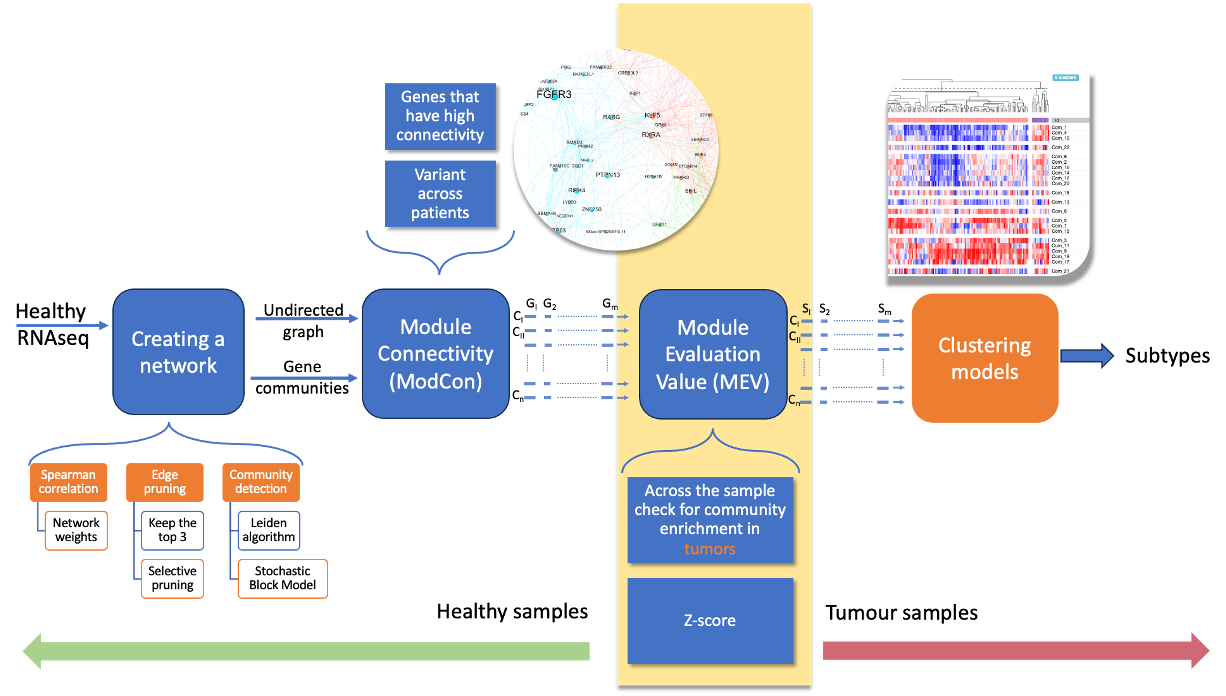
\includegraphics[width=0.95\textwidth,height=0.95\textheight,keepaspectratio]{Sections/Network_I/Resources/Methods/network_pipeline.png}
    \caption{Network pipeline}
    \label{fig:N_I:network_pipeline}
\end{sidewaysfigure}


% Start by giving an overview of the pipeline, there are several components to it: Network contruction & gene filtering, Community Detection, Finding the relevant genes in each community, Representation of this genes across samples & clustering
In Figure \ref{fig:N_I:network_pipeline} the network pipeline is broken in several stages 1) the network is constructed from RNA-seq data and to which community detection algorithms are applied 2) find the most important genes in each community and 3) find the representation of the genes from 3) to the samples and 4) apply clustering analysis to find the disease subgroups.

% Describe each componenet and why I'm doing this 

%% Gene filtering will be with Network Construction
\subsection{Gene filtering}
The genes are filtered by the same approach as in \cref{s:cs:methods}\footnote{This will be a reference to the Data pre-processing in the Clustering Analysis work with Interferon$\gamma$} selecting the top on either tje 4000 genes, for tumour networks \cref{s:N_I:tum}, or 5000 for P0 networks \cref{s:p0} forwith the highest median/standard deviation and which are expressed in at least 90\% of the samples. A Spearman Correlation matrix is then built on the 5K genes, where the correlation of two genes represents the edges' weight while network nodes are the genes themselves. 

% There is not specific rationale for choosing 3K or 5K top most varied genes. 
For clustering analysis usually a third of the expressed genes (3K-4K genes) are used (e.g. TCGA subtyping - \citet{Robertson2017-mg}). However, in the non-cancerous experiments it was observed that when selecting the top 3K most varied genes (in the non-tumour) there are just a few mutated in the tumour dataset, and 5K genes were used instead. Thus, the experiments are usually run with the number of genes ranging from 3K-5K; Graphs with 6K and 7K nodes (=genes) were also explored, but not included in this chapter as usually these networks were dense and even harder to analyse.

\subsection{Weight modifiers}

The network weights are modified to integrated the mutation burden across the TCGA cohort into the network. The changes are applied after the Spearman correlation matrix is computed but before the edge pruning. The reward strategy \textit{'promotes'} the genes which are highly mutated across tumours by increasing their weight, conversely the penalised strategy \textit{'punishes'} the genes that are highly mutated. The two modifiers are described in Figure \ref{fig:N_I:modifiers} where the highest mutated genes (e.g. \textit{TP53}, \textit{TTN}) are the most penalised/rewarded, while the weight values for un-mutated genes remain unchanged. It is worth mentioning, that there is no need to adapt the ModCon as the weight changes will affect the connectivity parameters from  \cref{eq:modcon}.

\begin{figure}[!htb]    
    \centering
    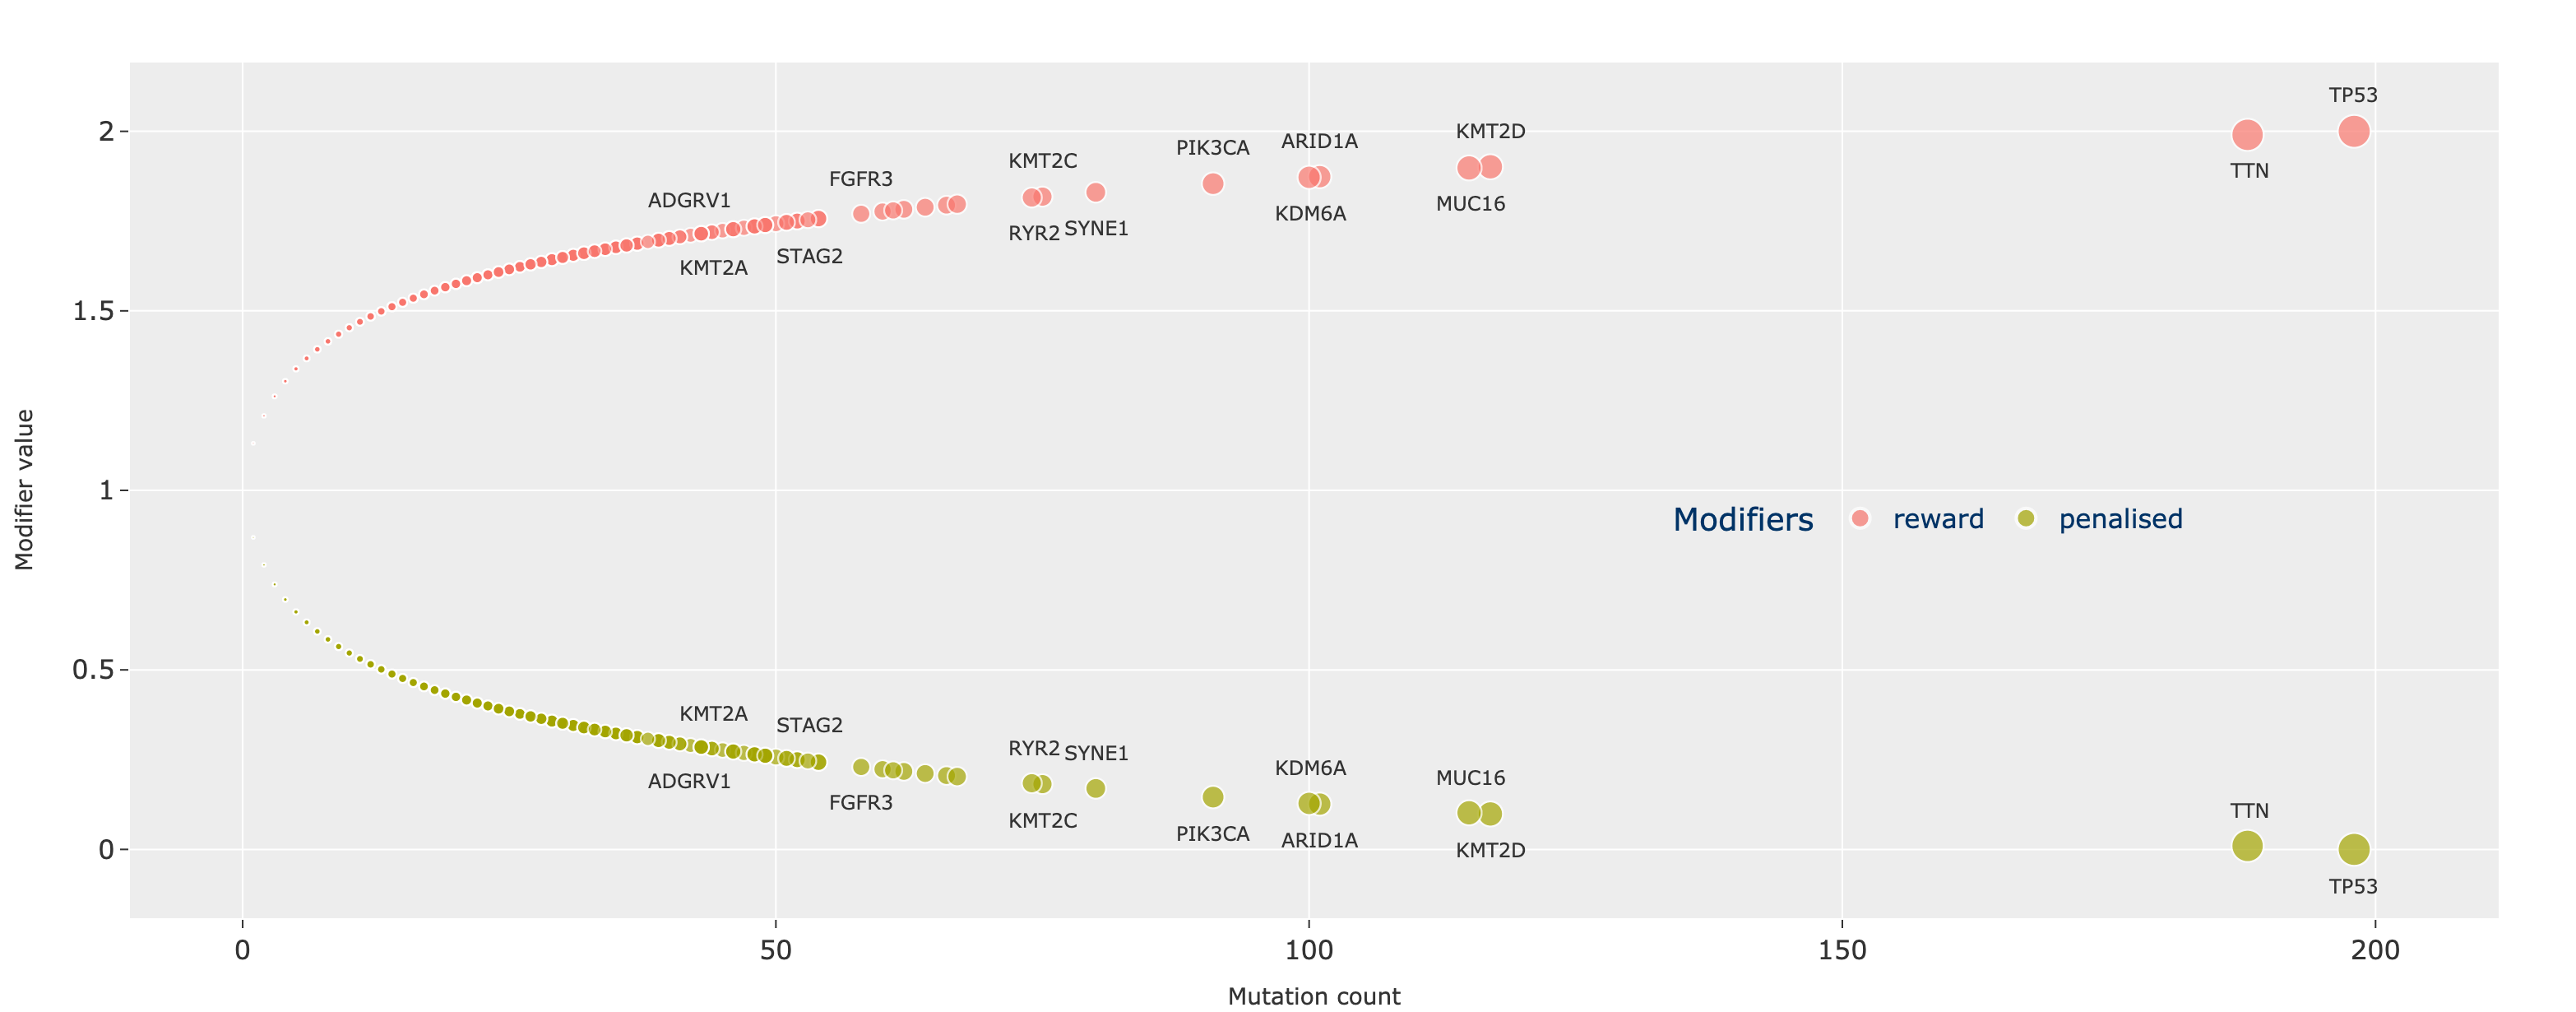
\includegraphics[width=1.0\textwidth,keepaspectratio]{Sections/Network_I/Resources/Methods/modifiers.png}
    \caption{Representing the two weight modifier strategies employed at the network construction stage. The red, reward strategy, awards the genes that have a high burden across the cohort. Conversely, the  penalised strategy decreases the edges' strength for highly mutated genes. In both cases, the non-mutated genes remain unchanged.}
    \label{fig:N_I:modifiers}
\end{figure}

% Selective edge pruning
\subsection{Edge pruning}

% Why there is a need for edge pruning
For a network of 5K nodes there are $1.24x10^6$ possible edges and keeping all of them makes the network challenging to analyse. In \citet{Care2019-ij} the authors explore different edge pruning strategies and found that on their datasets (Glioblastoma and Breast cancers) an aggressive strategy yields the best result. The strategy keeps the 3 top most correlated genes, meaning that each node has a minimum degree of 3. However, if gene A is in the top 3 of gene E, and the reverse is not true \footnote{Gene E is not in the top of gene A} then A will have a degree of 4 or the node has edges to the other 4 different genes. The authors from PGCNA build networks with 3-10 minimum edges for nodes and observed that the one with 3 edges yields the best result by the Modularity Score\footnote{Metric used by Leiden and Louivan algorithm to assess the community separation.} and the number of communities, where a larger number has the potential to yields better biological results.

The edge pruning approach from \citet{Care2019-ij} was implemented and adapted to have a preferential treatment for a list of genes that are Human Transcription Factors \citet{Lambert2018-el}. The TFs are genes that have a higher impact on the other genes by regulating their expression. Therefore, the selective edge pruning strategy developed would allow the TFs to have a higher number of edges compared to the standard genes. There are number of experiments performed on finding the right number of connections for TF genes in \cref{s:N_I:sel_pruning}.

% Community detection
\subsection{Community detection}

Once the network is built, a community detection algorithm is applied to find the sub-networks of genes. The purpose is to identify genes that are correlated with each other, which may potentially resemble some parts of the biological process. This hypothesis can be verified using Gene Set Enrichment Analysis (GSEA) or Gene Ontology (GO). It is worth noting that the ideal communities would be defined by biological pathways, but that information is often incomplete and not always available. Thus, the advantage of using a co-expressed network from mRNA gene expression is that it has the potential to be an affordable approximation.


In this project two main classes of community detection algorithms are explored: Leiden and Stochastic Block Model (SBM). The first algorithm is a popular method used to find partitions, blocks (=communities) used in the work of \citet{Care2019-ij}. However, Leiden may find non-existent structure in the data as explained in \citet{Peixoto2021-jx}. The SBM introduced by \citet{Peixoto2019-fg} addresses this issues by employing a Bayesian approach to find the blocks in the networks; both algorithms are covered in more depth in \cref{s:lit:comm_detect}.

In this project both methods are used. Initially, Leiden with Modularity Score is used in the Tumour (see \cref{s:N_I:tum}) and in P0 networks (see \cref{s:p0}). This is then followed by the experiments performed in the next chapter with all the non-tumour samples and the improved network pipeline in the last results chapter \cref{s:N_II}.

% Finding the relevant genes
\subsection{Important genes in communities}

In the work of \citet{Care2019-ij}, the  Module Connectivity (ModCon) score is computed for each gene to find the important nodes in each community (or Module). The equation can be found in \cref{eq:modcon} where $connectivity$ represents the sum of the genes' edges' weights, $percentileExpression$ is the gene's percentile expression, $VarWithin$ constitutes the median quantile coefficient of dispersion (or the gene expression dispersion within \textit{datasets}), $VarAcross$ is the "median absolute deviation of percentile expression" (or the gene dispersion across \textit{datasets}).

\begin{multline} \label{eq:modcon}
         ModCon = connectivity^2 \cdot percentileExpression \cdot VarWithin \\
         \cdot (100 - VarAcross) / 100
\end{multline}

The PGCNA was developed to support multiple datasets but in this project the majority of the experiments were run with a single dataset, thus $VarAcross$ does not have a large impact on \cref{eq:modcon}. Importantly, in the original formulation of $ModCon$, the connectivity parameter is the summation of the Spearman Correlation values. However, in the weight modifier experiments, where the Spearman Correlation values are strengthen/weaken by the gene's mutation burden the changed correlation are considered.

% Representation of genes across samples & Clustering
\subsection{Bridging the gap to samples} \label{s:N_I:mev}

After the genes are ranked by the importance in the nodes, the top 25-100 genes are selected as representative. The top 25 genes were selected in PGCNA work \citep{Care2019-ij} which worked when the same dataset is used for network and subtyping. However, when the non-tumour graphs were computed, there are situations when the most varied genes in the non-cancerous dataset are not present in the tumours dataset. Thus, more genes (100) were selected for each community. These chosen genes are used to compute the Module Evaluation (MEV) score \citep{Care2019-ij} to find the gene's representation in each of the samples. The MEV is described in the pseudo-code in \cref{alg:N_I:mev}.

\begin{algorithm}
\caption{Module Evaluation Value }\label{alg:N_I:mev}
    \begin{algorithmic}
    \For{each community in all the network communities}     
        \For{each gene in the top selected genes} 
            \State $z\_score=$ for the quantile normalised $log2$(gene expression)
            \For{each patient in all samples}  
                \State $MEV=$ sum of the z-score  \Comment{Only for the top selected genes}
            \EndFor
        \EndFor
    \EndFor
    \end{algorithmic}
\end{algorithm}

The output of the \cref{alg:N_I:mev} is a $MxN$ matrix, where $M$ is the number of communities and $N$ the number of samples in the targeted dataset. On this matrix clustering analysis can then be applied to find the cancer subtypes. Thus, the methods and analysis tools developed in the previous chapter on cluster analysis,\cref{s:clustering_analysis}, can be applied to find the appropriate cluster configuration (see \cref{s:p0:clustering_analysis}).


\subsection{Implementation details} \label{s:N_I:implementation}

The experiments performed in this section are using a modified version of the PGCNA packaged developed by \citet{Care2019-ij}. It is worth noting that PGCNA was developed to support gene expression integration at the network level i.e., use the median expression across the given datasets. For the needs of the project this was not needed and a single gene expression is used to created the networks but with the new data integration. 

% Changes made
Initially the correlation values between genes is changed based on the weight modifiers proposed in \cref{fig:N_I:modifiers} and their effect are explored in both tumour and P0 networks in \cref{s:N_I:tum,s:p0}. Then, the number of edges is selectively altered for a given subset of genes (i.e., TFs) and the experiments for this are covered in \cref{s:N_I:sel_pruning}. 